\subsection{Nesymetrické napájení}
    \begin{figure}[h!]
        \centering
        \includegraphics[width=\textwidth]{microcap/Nesym/1.png}
        \centering
        \caption{Stejosměrný pracovní bod zapojení s nesymetrickým napájením.}
        \label{fig:ns-s-pracBod}
    \end{figure}

    \begin{figure}[h!]
        \centering
        \includegraphics[width=\textwidth]{microcap/Nesym/2.png}
        \centering
        \caption{Střídavé poměry v obvodu, vliv vazebních kondenzátorů na vstupu a výstupu obvodu. Horní průběh -- stejnosměrně posunutý vstup a výstup OZ kvůli kompenzaci nesymetrického napájení.}
        \label{fig:ns-s-prubeh1}
    \end{figure}

    \begin{figure}[h!]
        \centering
        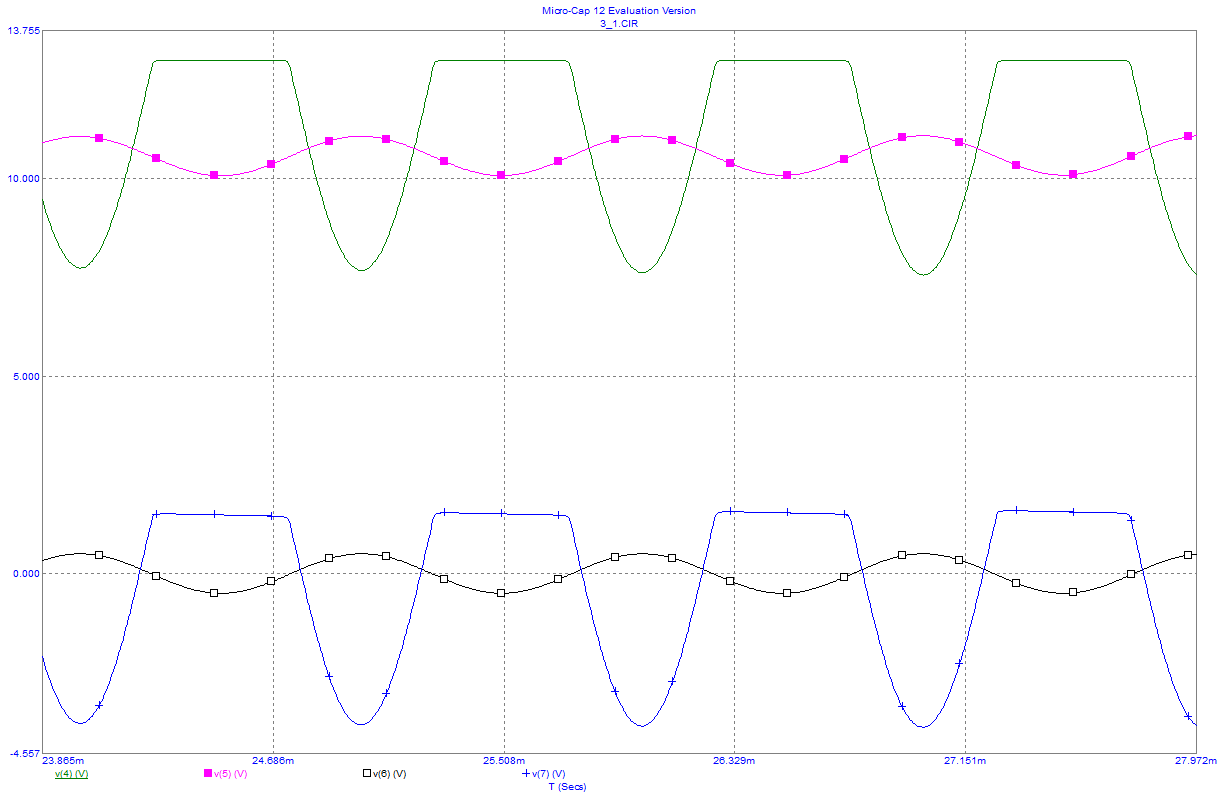
\includegraphics[width=\textwidth]{microcap/Nesym/3-r4-56k.png}
        \centering
        \caption{Změna poměru odporového děliče ($R_4=\qty{56}{\kilo\ohm}$), vyšší stejnosměrné posunutí vede k dosažení saturačního napětí.}
        \label{fig:}
    \end{figure}

    \begin{figure}[h!]
        \centering
        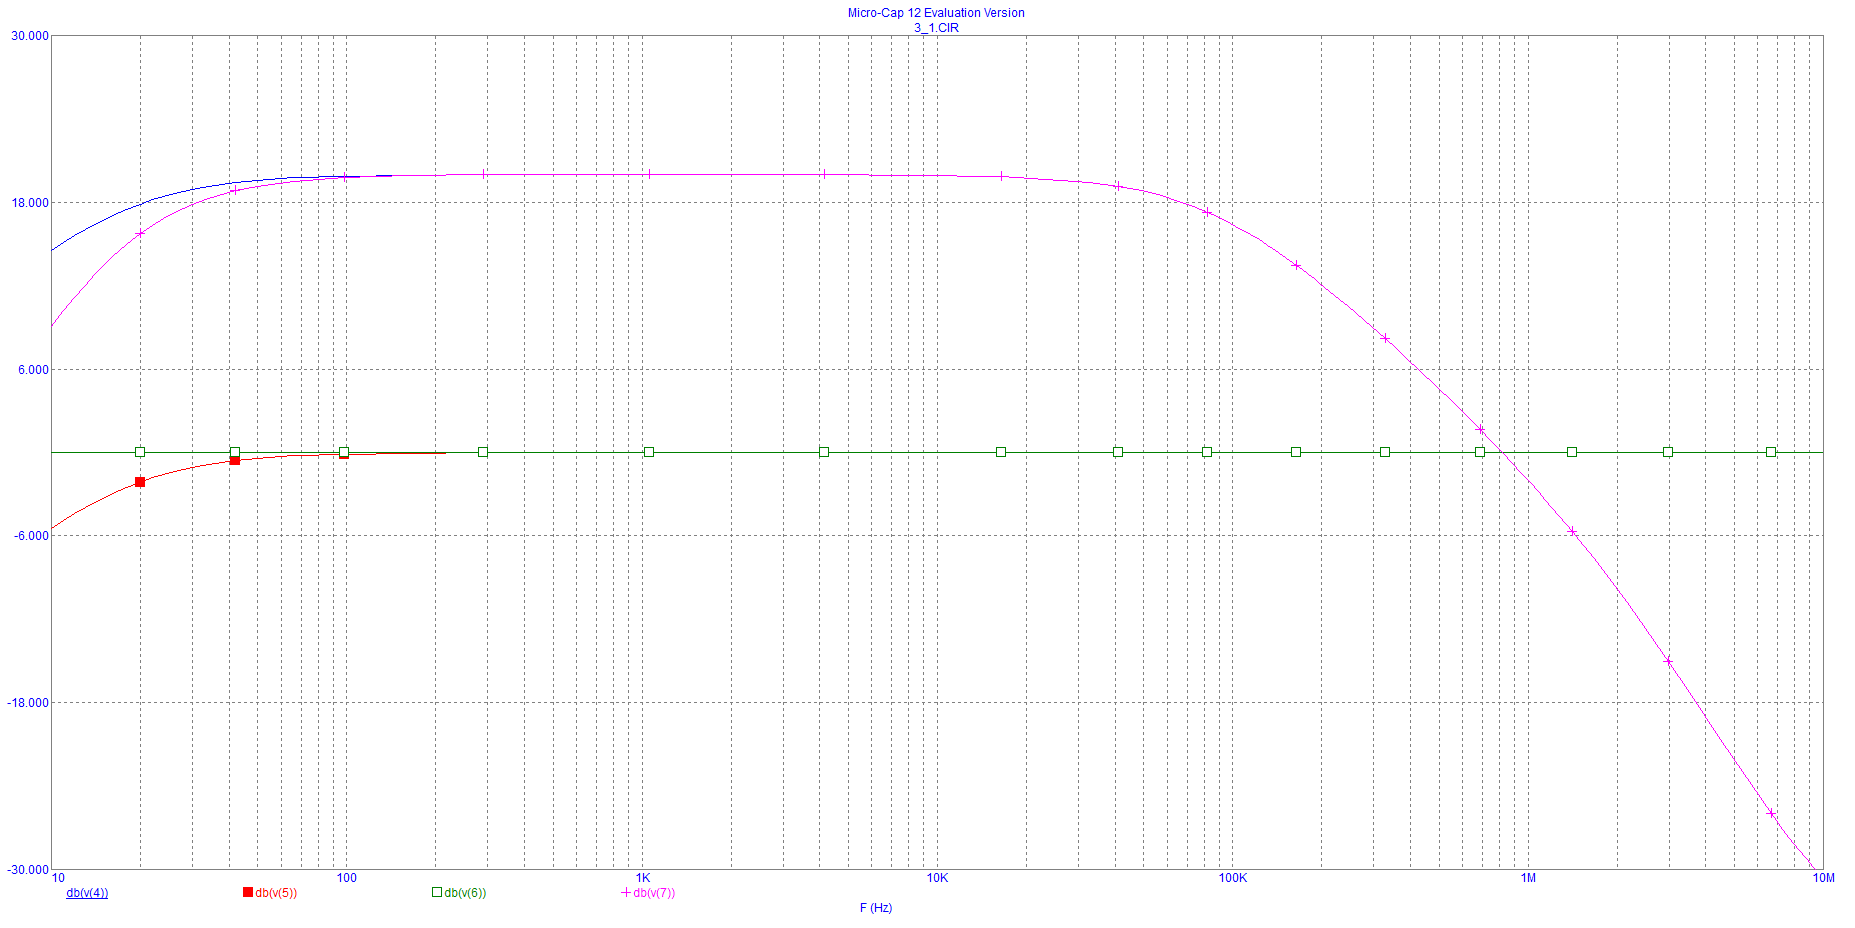
\includegraphics[width=\textwidth]{microcap/Nesym/4.png}
        \centering
        \caption{Amplitudová kmitočtová charakteristika přenosu napětí do jednotlivých uzlů. Modrá, červená, zelená a fialová jsou po řadě uzly 4-7.}
        \label{fig:}
    \end{figure}


\clearpage
\subsection{Sumační zesilovač}
        \begin{figure}[h!]
            \centering
            \includegraphics[width=\textwidth]{microcap/Sumac/1.png}
            \centering
            \caption{Stejnosměrný pracovní bod v zapojení sumačního zesilovače.}
            \label{fig:}
        \end{figure}

        \begin{figure}[h!]
            \centering
            \includegraphics[width=\textwidth]{microcap/Sumac/2.png}
            \centering
            \caption{Simulace součtu dvou vstupních signálů na výstupu OZ, výstup je navíc invertovaný.}
            \label{fig:}
        \end{figure}

\clearpage
\subsection{Rozdílový zesilovač}
    \begin{figure}[h!]
        \centering
        \includegraphics[width=\textwidth]{microcap/Difer/1.png}
        \centering
        \caption{Stejnosměrný pracovní bod v zapojení rozdílového zesilovače.}
        \label{fig:}
    \end{figure}

    \begin{figure}[h!]
        \centering
        \includegraphics[width=\textwidth]{microcap/Difer/2.png}
        \centering
        \caption{Simulace odečtení jednoho vstupního signálu od druhého, signál na výstupu OZ je navíc invertovaný.}
        \label{fig:}
    \end{figure}

    \begin{figure}[h!]
        \centering
        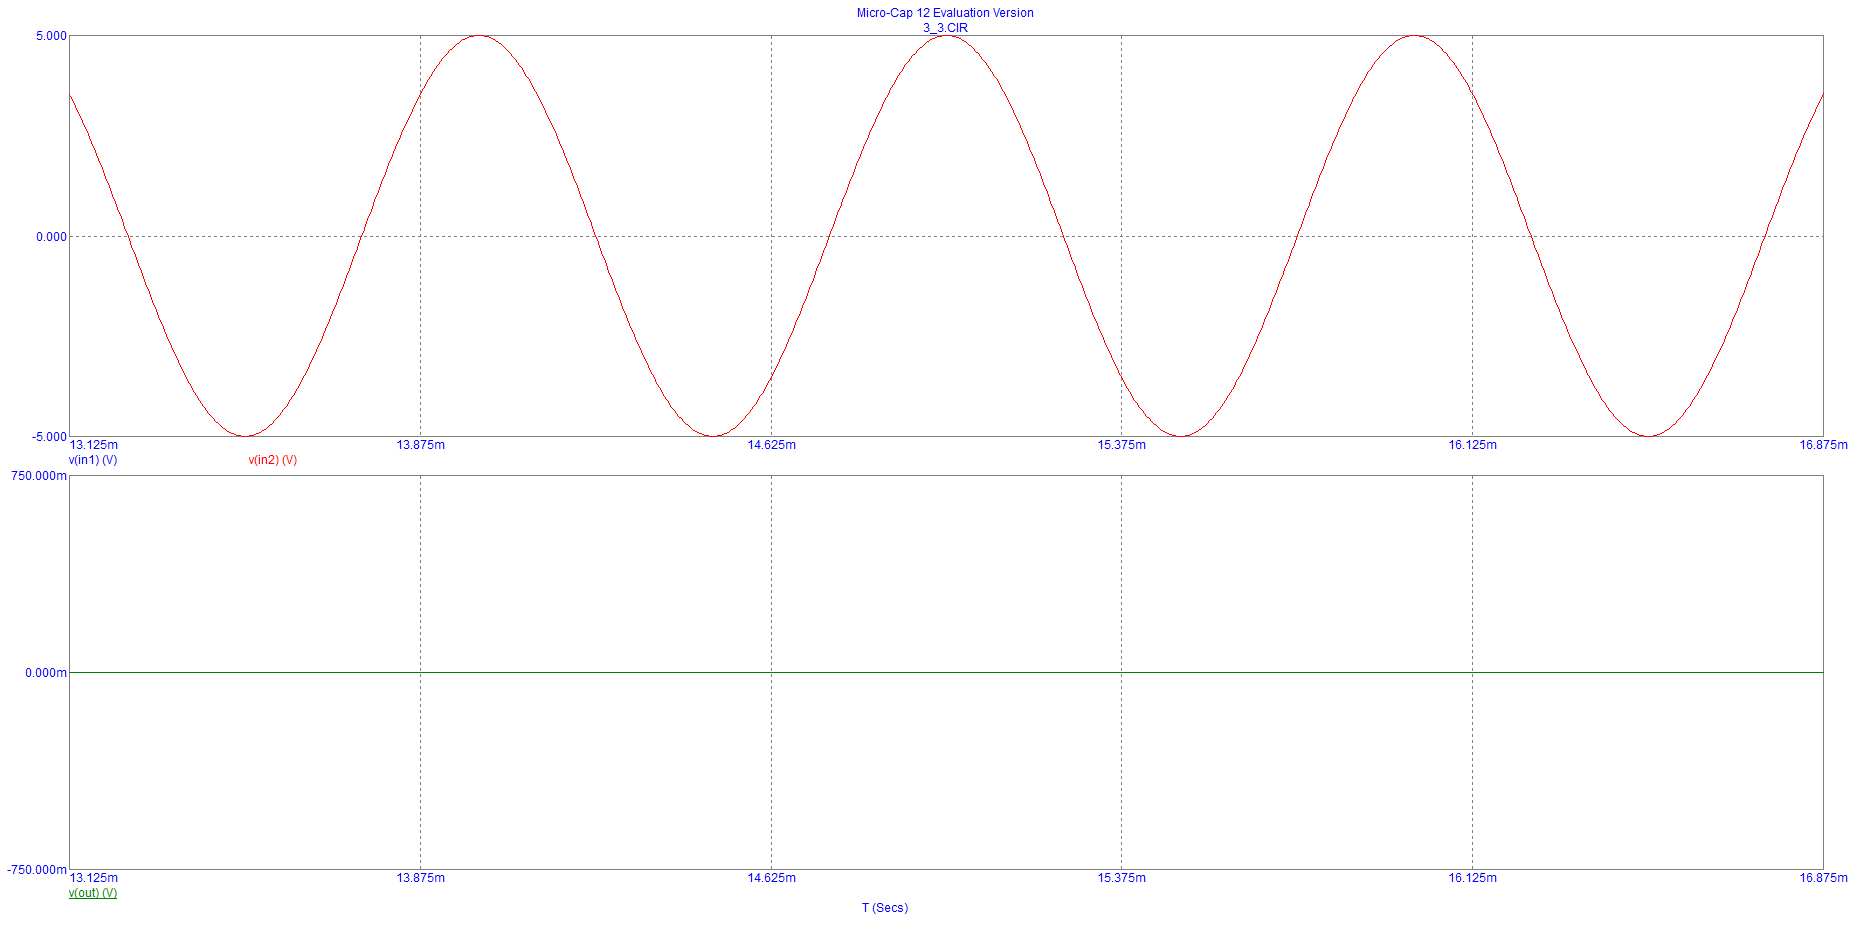
\includegraphics[width=\textwidth]{microcap/Difer/3.png}
        \centering
        \caption{Simulace odečtení dvou stejných signálů (zobrazeny přes sebe), na výstupu je signál nulový.}
        \label{fig:}
    \end{figure}
